\chapter{Preliminaries}

\section{Introduction}

This chapter presents a brief idea concerning the core concepts of 
smart farming system, which is able to recognize plant type, plant 
disease, ripeness stage and recommend, fertilizers, herbicides, and 
insecticides. Then it presents a brief idea about deep learning, 
and transfer learning.


\section{Smart Agriculture System}
Smart farming is a new concept that makes agriculture more efficient
and effective using advanced information technologies. The latest 
advancements in connectivity, automation, and artificial intelligence
enable farmers better to monitor all procedures and apply precise 
treatments determined by machines with superhuman accuracy. Farmers, 
data scientists, and engineers continue to work on techniques that allow 
for optimizing the human labor required in farming. With valuable information 
resources, improving daily, smart farming becomes a learning system and even 
more intelligent \cite{una20}. \\

Plants are a pivotal part of our planet. Because of the existence of plants, 
the earth is called a green planet. They play a fundamental role in our life. 
To understand, we can't imagine our life without oxygen which plants provide, 
in addition to the relation of plants to our food, medicines, and furniture. 
Accordingly, we can say that plants were the basis of life. Plants are divided 
into smaller groups according to shared attributes. Plants recognition is complicated 
because plants are highly complex. The recognition process of familiar plants was easy 
for experts. Sometimes, especially in medicine, we need to identify prejudiced or toxic 
plants, botanists can do that facilely, but they must find a way to categorize the different 
species when there are millions of various plant species, which are composed of similar parts 
(roots, stems, leaves, etc.). Designing a plant recognition system is required to save time 
and decrease cost \cite{has18}. \\

Early detection of plant disease is crucial to keep a crop healthy. 
The identification of plant disease can be a tedious task in many parts of 
the world due to the unavailability of the required equipment. Moreover, 
it has been reported that diseases and pests can reduce yields by more than 
50\%, and small farmers are the most vulnerable to this issue. For efficient 
crop management, the correct identification of the disease should be fast and cheap. 
With the huge leap in technological advancement in the past few years, high-resolution 
cameras, smartphones, and computers have become widespread and accessible to a large 
portion of the population \cite{moh16}.
All these factors can make an automated solution feasible, especially since deep learning 
techniques have shown their ability to perform exceptionally well on complex tasks. 
Early detection of plant diseases can help farmers effectively monitor the health of 
their culture in addition to make the best decision to avoid the spread of pathogens \cite{mas21}.
Figure (\ref{fig:framework}) shows the general framework of Smart Agriculture System.

\begin{figure}[H]
    \centering
    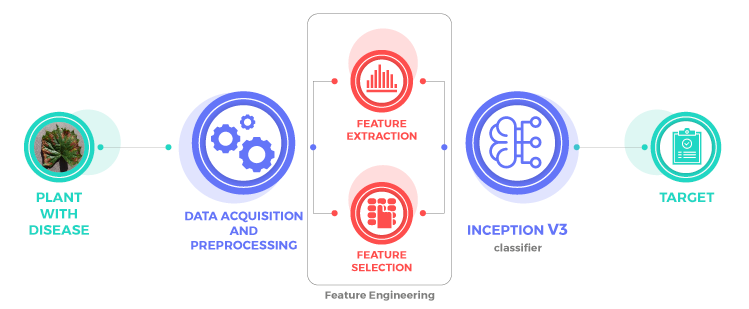
\includegraphics[width=14cm]{photos/chapter03/1.png}
    \caption{General framework of Smart Agriculture System}
    \label{fig:framework}
\end{figure}

Moreover, Monitoring and controlling fruits and vegetables ripeness has become a 
very important issue in the crops industry, since ripeness is perceived by customers 
as the main quality indicator. Also, the product's appearance is one of the most worrying 
issues for producers as it has a high influence on product's quality and consumer preferences. 
However, up to this day, optimal harvest dates and prediction of storage life are still mainly 
based on subjective interpretation and practical experience. A standard smart farming system 
comprises three major components as depicted in Figure (\ref{fig:framework}). \\

{\bf Data acquisition and preprocessing phase} constitute a very important phase 
of any intelligent damage detection system and have a significant influence on 
the capability for damage detection and assessment. It is responsible for data 
collecting using various sensors and preprocessed the collected data for the 
feature engineering phase. Preprocessing includes data cleaning, data 
transformation, and dimension reduction. \\

{\bf Feature engineering phase} is the key component of a successful ML algorithm, 
contributing to their performance. It aims to extract features that better 
represent the underlying problem from raw data and transforming them into 
a proper format for machine learning models. \\

{\bf Classification phase} is responsible for classifying patterns into various 
categories using ML algorithms. These algorithms can be classified into three 
categories, namely, supervised learning, semi-supervised learning, and 
unsupervised learning based on the amount of required labeled data \cite{esr20}.


\section{Data Preprocessing}

\subsection{Data augmentation}
The high performance of deep CNN models is dependent on the availability 
of a large amount of training data. Unfortunately, a major issue generally 
faced by DL or ML is the scarcity of training data. As a result of insufficient 
training data, classification models suffer from the overfitting problem. To 
overcome the problem of overfitting, different regularization technologies are used, 
such as batch normalization and dropout layer usage. Another smart solution to this 
problem is data augmentation. It is the process of generating new samples that are 
similar to the training samples. However, unluckily, choosing inappropriate data 
augmentation methods is likely to lead to augment samples that are not sufficiently 
informative, which result in no impact or detrimental impact on the classifier's accuracy and 
robustness. Therefore, selecting the most appropriate data augmentation method according to the 
nature and requirements of the studied problem is key in achieving higher accuracy and robustness 
of classifiers, with a restricted number of generated training samples \cite{esr20}.

\subsection{Feature Engineering}
Feature Engineering is defined as the process of extracting features that better 
represent the underlying problem from raw data and transforming them into a suitable 
format for machine learning models, resulting in improving the performance of a trained 
model on unseen data. Feature engineering can be categorized into two categories, namely, 
feature extraction and feature selection. The main aim of feature extraction and selection is to
\begin{enumerate}
    \item Reduce high-dimensional feature space to low-dimensional representation.
    \item Focus on the most relevant data.
    \item A void overfitting the data.
    \item Improve the quality of feature space and hence the performance of machine
        learning algorithms such as learning time and accuracy \cite{esr20}.
\end{enumerate}

\subsection{Feature Extraction}
Feature extraction is the process of extracting a set of new features from the original 
features through some mapping functions. Feature extraction methods can be practically 
classified into three groups: \cite{esr20}
\begin{enumerate}
    \item The hand-crafted features.
    \item The learned ones.
    \item hybrid features.
\end{enumerate}

\textbf{Hand-crafted features} are those, which are extracted from an image following some 
certain hand-engineered predefined algorithms based on expert knowledge. There are 
a wide variety of state-of-the-art algorithms for the hand-crafted features.
In contrast to the hand-crafted features, the \textbf{learned ones} are those set 
of features that are learned directly from raw input images by training a network 
with a labeled dataset to accomplish a certain task (e.g. face recognition). 
Convolutional Neural Networks (CNNs) are considered main examples of deep 
neural networks (DNNs), which can be used to extract learned features. The 
main idea behind the learned features approach is to discover data 
representations with multiple levels of abstraction to enable higher-level
features of representing the semantics of the data, which provides better 
robustness to intra-class variability. Finally, hybrid features are those 
set of features that integrate both hand-crafted and learned features. 
In this chapter, we shall briefly discuss some of the popular learned 
features and hand-crafted features used in building SHM systems \cite{esr20}.

\section{Deep Learning}

In the last few years, the deep learning (DL) computing paradigm has been 
deemed the Gold Standard in the machine learning (ML) community. Moreover,
it has gradually become the most widely used computational approach in the 
field of ML, thus achieving outstanding results on several complex cognitive 
tasks, matching or even beating those provided by human performance. One of 
the benefits of DL is the ability to learn massive amounts of data. The DL 
field has grown fast in the last few years and it has been extensively used 
to successfully address a wide range of traditional applications. More 
importantly, DL has outperformed well-known ML techniques in many domains, 
e.g., cybersecurity, natural language processing, bioinformatics, robotics 
and control, and medical information processing, among many others. Despite 
it has been contributed several works reviewing the State-of-the-Art on DL, 
all of them only tackled one aspect of the DL, which leads to an overall 
lack of knowledge about it \cite{alz21}.

\subsection{Convolutional Neural Networks (CNNs)}
Among the various deep neural network models, CNN is considered the most 
commonly used model for image classification. Standard CNN consists of 
several convolutional layers, pooling layers, and fully-connected (FC) 
layers. Figure (3.2) shows an example of CNN architecture. The main aim 
of the CNN is the automatic and adaptive learning of spatial hierarchies 
of useful features, from low-to high-level patterns \cite{esr20}.
Figure (\ref{fig:CNNArch}) shows an example of CNN architecture.

\begin{figure}[H]
    \centering
    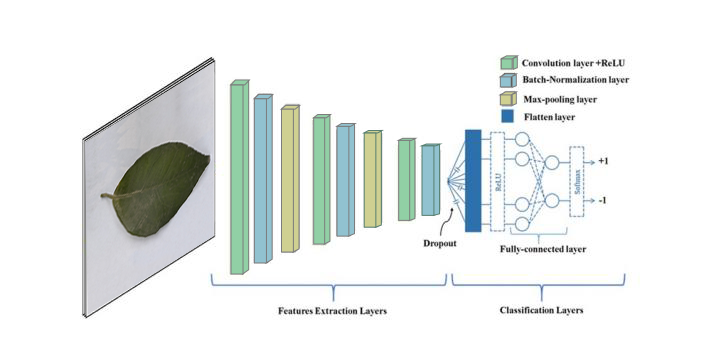
\includegraphics[height=70mm]{photos/chapter03/2.png}
    \caption{An example of CNN architecture.}
    \label{fig:CNNArch}
\end{figure}

\begin{enumerate}
    \item {\bf Convolutional Layer:} \\[5pt]
        The convolutional layer is the key aspect of CNN. Given an input 
        array A of size I a receptive field, and stride step $N$, it operates 
        by applying three steps. The first step is an element-by-element 
        multiplication between a sub-array of A, and a receptive field 
        (both of size $N x N$). The second step is the summation of the 
        multiplied values and adding bias to the summed values. The 
        final step adds the final values to the output array. The 
        receptive field is also often called the filter, or kernel. 
        The weight values of a receptive field are initialized randomly \cite{esr20}.

    \item {\bf Pooling Layer:} \\[5pt]
        Another key aspect of CNN is the down-sampling process performed by 
        the pooling layer. It aims to achieve spatial invariance by reducing 
        the resolution of the input feature map. Each pooled feature map 
        corresponds to one feature map of the previous layer. Max and mean 
        pooling are two types of pooling. The maximum values from an input 
        array's sub-arrays are taken in max-pooling, while in mean pooling 
        the mean values are taken. From the survey, max-pooling performance 
        in image datasets outperformed mean pooling \cite{esr20}.

    \item {\bf Activation Layer:} \\[5pt]
        The activation layer is a non-linear transformation function, widely 
        used in the standard Artificial Neural Networks {\bf (ANN)}. There are many 
        different activation functions such as sigmoid, hyperbolic tangent $(tanh)$, 
        Rectified Linear Unit ({\bf ReLU}), etc. It is applied after the convolution operation 
        is completed to enable CNNs to avoid learning trivial linear combinations of inputs. 
        All non-linear functions are restricted to output values except {\bf ReLU}, which has only 
        restricted outputs for its negative inputs. The features of {\bf ReLU} make computation faster 
        and more accurate. {\bf ReLU} is computed according to equation (\ref{eq:activation}) \cite{esr20}.
        \begin{equation} \label{eq:activation}
            R(z) \ = \ max(0, z)
        \end{equation}
        Where $z$ is the input to a neuron.

    \item {\bf Softmax Layer:} \\[5pt]
        For classifying input image, having a layer for prediction is necessary matter. 
        This layer is responsible for classifying input images and is located at the end 
        of CNN model. It can be any machine learning algorithms such as support vector machine 
        {\bf (SVM)}, multilayer perceptron {\bf (MLP)}, etc. To date, using softmax function given by 
        equation (\ref{eq:softmax}) is the most outstanding method \cite{esr20}. 
        \begin{equation} \label{eq:softmax}
            yk \ = \ \exp(\phi \ k) \ / \ (j \ \exp(\phi \ j)) 
        \end{equation}
        Where $\phi$ is the neural network outputs and $y$ is the probability of belonging to a class.
\end{enumerate}

\subsection{The Used CNN Deep Learning Model}
{\bf There are various CNN models such as} LeNet, AlexNet, ResNet, 
GoogleNet / InceptionNet, Depth based CNNs, VGG, Inception v2, 
Inception v3, Inception-ResNet, DenseNet, etc. Inception v3 
deep learning model was selected because it is the advanced 
and optimized version of the inception V1 model. The Inception 
V3 model used several techniques for optimizing the network for 
better model adaptation \cite{rat18}.
\begin{itemize}
    \item It has higher efficiency.
    \item It has a deeper network compared to the Inception V1 and V2 models, but its speed isn't compromised.
    \item It uses auxiliary Classifiers as regularizes \cite{sam19}.
\end{itemize}

\subsection{Inception v3}
Inception V3 by Google is the $3^{rd}$ version in a series of Deep 
Learning Convolutional Architectures \cite{bar19}. It is mainly focuses 
on burning less computational power by modifying the previous 
Inception architectures and an image recognition model that 
has been shown to attain greater than 78.1\% accuracy on the
ImageNet dataset. The model is the culmination of many ideas 
developed by multiple researchers over the years. Figure (\ref{fig:incv3})
shows the structure of Inception V3 model.

\begin{figure}[H]
    \centering
    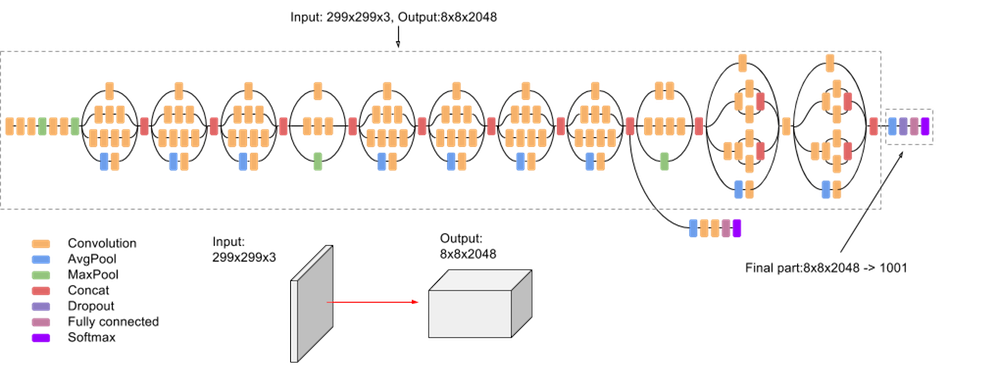
\includegraphics[height=58mm]{photos/chapter03/3.png}
    \caption{Structure of Inception V3 model.}
    \label{fig:incv3}
\end{figure}

\noindent The model itself is made up of symmetric and asymmetric building blocks, 
including convolutions, average pooling, max pooling, concatenations, 
dropouts, and fully connected layers. Batch normalization is used extensively 
throughout the model and applied to activation inputs. Loss is computed using Softmax \cite{dem19}.

\subsection{Yolov5}
YOLO is an acronym that stands for You Only Look Once. 
used Version 5, which was launched by Ultralytics in June 2020 and is now the 
most advanced object identification algorithm available due to its speed and accuracy. 
It is a novel convolutional neural network (CNN) that detects objects in real-time with 
great accuracy. This approach uses a single neural network to process the entire picture, 
then separates it into parts and predicts bounding boxes and probabilities for each 
component. These bounding boxes are weighted by the expected probability. The method 
"just looks once" at the image in the sense that it makes predictions after only one 
forward propagation run through the neural network. It then delivers detected items 
after non-max suppression (which ensures that the object detection algorithm only identifies each object once). 
Figure (\ref{fig:yolov5}) shows scheme of the YOLOv5 architecture.
\begin{figure}[H]
    \centering
    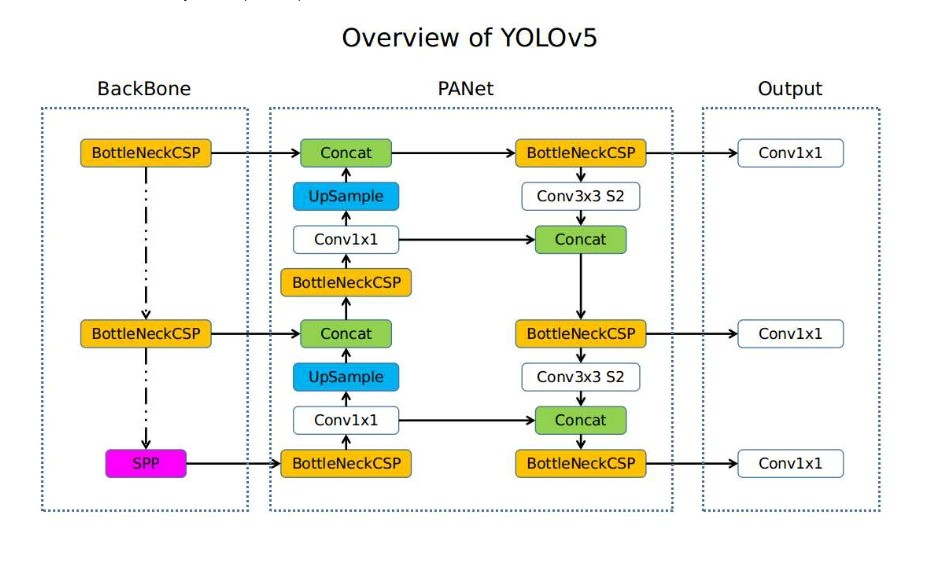
\includegraphics[height=85mm]{photos/chapter03/4.jpg}
    \caption{Scheme of the YOLOv5 Architecture.}
    \label{fig:yolov5}
\end{figure}
The model itself is made up of symmetric and asymmetric building blocks, 
including convolutions, average pooling, max pooling, concatenations, 
dropouts, and fully connected layers. Batch normalization is used extensively 
throughout the model and applied to activation inputs. Loss is computed using Softmax \cite{dem19}.
\begin{enumerate}
    \item {\bf Backbone:} Model Backbone is mostly used to extract key features from an input 
        image. CSP (Cross Stage Partial Networks) are used as a backbone in YOLO v5 to
        extract rich in useful characteristics from an input image.
    \item {\bf Neck:} The Model Neck is mostly used to create feature pyramids. 
        Feature pyramids aid models in generalizing successfully when it comes to 
        object scaling. It aids in the identification of the same object in various 
        sizes and scales. Feature pyramids are quite beneficial in assisting models 
        to perform effectively on previously unseen data. Other models, such as FPN, 
        BiFPN, and PANet, use various sorts of feature pyramid approaches.
        PANet is used as a neck in YOLO v5 to get feature pyramids.
    \item {\bf Head:} The model Head is mostly responsible for the final detection step. 
        It uses anchor boxes to construct final output vectors with class probabilities, 
        objectness scores, and bounding boxes \cite{gar21}.
\end{enumerate}

\section{Transfer Learning}

Transfer learning is an emerging topic that may drive the success of 
machine learning in research and industry. The lack of data on specific 
tasks is one of the main reasons to use it, since collecting and labeling 
data can be very expensive and can take time, and recent concerns with 
privacy make difficult to use real data from users. The use of transfer 
learning helps to fast prototype new machine learning models using pre-trained 
models from a source task since training on millions of images can take time 
and requires expensive GPUs \cite{rib19}.

\subsubsection{Step by step transfer learning process}

\begin{enumerate}
    \item {\bf Obtain pre-trained model:} \\[3pt]
        The first step is to choose the pre-trained model we would like to 
        keep as the base of our training, depending on the task. Transfer 
        learning requires a strong correlation between the knowledge of 
        the pre-trained source model and the target task domain for them 
        to be compatible. \\
        Here are some of the pre-trained models you can 
        use: VGG-16, VGG-19, Inception V3, XCeption, ResNet-50, and etc.

    \item {\bf Create a base model:} \\[3pt]
        The base model is one of the architectures such as ResNet or Xception which 
        we have selected in the first step to be in close relation to our task. We can 
        either download the network weights which saves the time of additional training 
        of the model. Else, we will have to use the network architecture to train our 
        model from scratch. There can be a case where the base model will have more 
        neurons in the final output layer than we require in our use case. In such 
        scenarios, we need to remove the final output layer and change it accordingly.

    \item {\bf Freeze layers:} \\[3pt]
        Freezing the starting layers from the pre-trained model is essential to 
        avoid the additional work of making the model learn the basic features.
        If we do not freeze the initial layers, we will lose all the learning 
        that has already taken place. This will be no different from training 
        the model from scratch and will be a loss of time, resources, etc. \\\\

    \item {\bf Add new trainable layers:} \\[3pt]
        The only knowledge we are reusing from the base model is the feature 
        extraction layers. And add additional layers on top of them to predict 
        the specialized tasks of the model. These are generally the final output layers.

    \item {\bf Train the new layers:} \\[3pt]
        The pre-trained model's final output will most likely differ from the output of 
        model. For example, pre-trained models trained on the ImageNet dataset will output 
        1000 classes. However, need model to work for two classes. In this case, have to 
        train the model with a new output layer in place.

    \item {\bf Fine-tune your model:} \\[3pt]
        One method of improving the performance is fine-tuning. Fine-tuning involves 
        unfreezing some part of the base model and training the entire model again on 
        the whole dataset at a very low learning rate. The low learning rate will 
        increase the performance of the model on the new dataset while preventing 
        overfitting \cite{v7lab}.
\end{enumerate}
